% Source: Wald GR, physical PDF p. 169
%         (printed p. 156).
% Coverage: Figure 6.11, complete gravitational collapse.
% Figures/tables/footnotes: Figure 6.11; no tables or footnotes.
% Status: source-reviewed and compile-clean.
% Uncertainties: none.
\begingroup
\renewcommand{\thefigure}{6.11}
\begin{figure}[htbp]
\centering
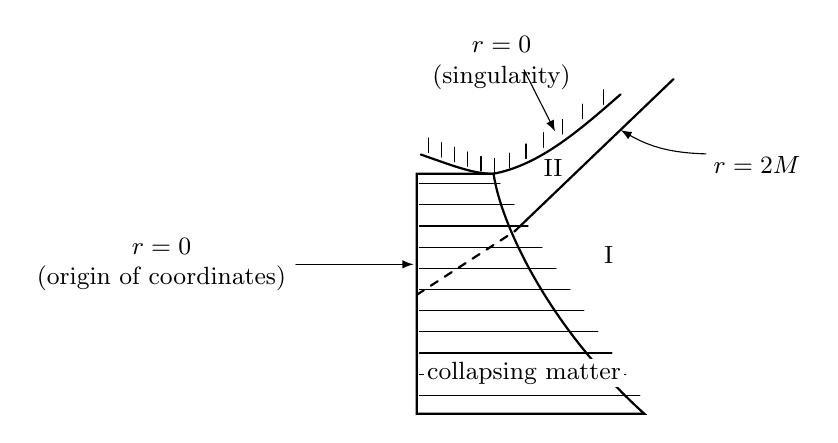
\begin{tikzpicture}[scale=.84,>=latex,font=\small,line cap=round]
  % World tube of the matter: the left edge is the regular center r=0 and
  % the right edge shrinks as the body collapses.
  \draw[thick] (-1.72,-2.58) -- (-1.72,1.05) -- (-.56,1.05)
    .. controls (-.45,.28) and (.28,-1.28) .. (1.72,-2.58) -- cycle;
  \foreach \y in {-2.30,-1.98,-1.66,-1.34,-1.02,-.70,-.38,-.06,.26,.58,.90} {
    \draw[thin] (-1.68,\y) -- ({-.56+.66*(1.05-\y)},\y);
  }
  % Event horizon: dashed while it lies inside the matter, solid outside.
  \draw[dashed,thick] (-1.72,-.78) -- (-.24,.18);
  \draw[thick] (-.24,.18) -- (2.16,2.48);
  % The future spacelike singularity.
  \draw[thick] (-1.66,1.34) .. controls (-1.20,1.18) and (-.85,1.04) .. (-.56,1.05)
    .. controls (.12,1.18) and (.70,1.67) .. (1.36,2.25);
  \foreach \x/\y in {-1.55/1.37,-1.35/1.30,-1.15/1.23,-.95/1.16,-.75/1.09,
      -.55/1.06,-.32/1.14,-.07/1.28,.20/1.45,.48/1.65,.78/1.88,1.10/2.10} {
    \draw (\x,\y) -- ++(0,.22);
  }
  \draw[->] (2.65,1.35) to[bend left=14] (1.36,1.71);
  \node[right] at (2.62,1.18) {\(r=2M\)};
  \draw[->] (-3.55,-.32) -- (-1.77,-.32);
  \node[align=center,anchor=east] at (-3.55,-.32) {\(r=0\)\\(origin of coordinates)};
  \draw[->] (-.10,2.62) -- (.37,1.69);
  \node[align=center] at (-.44,2.72) {\(r=0\)\\(singularity)};
  \node[fill=white,inner sep=1pt] at (-.10,-1.96) {collapsing matter};
  \node at (1.18,-.18) {I};
  \node at (.34,1.13) {II};
\end{tikzpicture}
\caption{The spacetime resulting from the complete gravitational collapse of a
spherical body. All of regions III and IV of the extended Schwarzschild
spacetime (Figure~\ref{fig:6.9}) are covered up by the collapsing matter.
However, part of the black hole region II is produced.}
\label{fig:6.11}
\end{figure}
\endgroup
